It is obvious that
	\begin{align}
		\vec{n} 
			= \vec{e}_2,
	\vec{c} =\vec{u}=\vec{0}.
\end{align}
Consequently,
%
\begin{align}
	\vec{V} &= \myvec{1 &0\\ 0 & 1-e^2}
	\\
	\vec{F} &= ce^2\vec{e}_2 \implies \norm{\vec{F}} = ce^2=8
\label{eq:chapters/11/11/4/8/F}
	\\
	f 
	  &= 64 - c^2 e^2
\label{eq:chapters/11/11/4/8/f}
\end{align}
%
Since the vertices are  on the conic,
\begin{align}
	\vec{v_1}^{\top}\vec{V}\vec{v_1} +2\vec{u}^{\top}\vec{v_1}+f &= 0\\
\implies 25\brak{1-e^2} + f &= 0\\
	 \label{eq:chapters/11/11/4/8/1}
\end{align}
Solving \eqref{eq:chapters/11/11/4/8/1},
\eqref{eq:chapters/11/11/4/8/F}
and
\eqref{eq:chapters/11/11/4/8/f},
\begin{align}
	c = \frac{9}{5},\ 
	e = \frac{5}{3},
\end{align}
%
yielding
\begin{align}
	\vec{V} = \myvec{1&0\\0& -\frac{16}{9}} ,\
	\vec{u} = \myvec{0\\0},\
	f = 16.
\end{align}
%
Thus, the desired equation of the hyperbola is
\begin{align}
	\vec{x}^{\top} \myvec{1&0\\ 0 & -\frac{16}{9}} \vec{x} +16 =0
\end{align}
%
\item We know the Focii is given as
\begin{align}
	\vec{F} &= \pm \frac{\brak{\frac{1}{e\sqrt{1-e^2}}}\brak{e^2}\sqrt{\frac{\lambda_1}{f_0}}}{\frac{\lambda_1}{f_0}}\vec{e}_2\\
	        &= \frac{\frac{e}{\sqrt{1-e^2}}}{\sqrt{\frac{\lambda_1}{f_0}}}\vec{e}_2
\end{align}
Substituting \eqref{eq:chapters/11/11/4/8/eq1} we get
\begin{align}
	\vec{F} &= 5e\vec{e}_2\\
	\myvec{0\\8} &= 5e\vec{e}_2\\
	\implies e &= \frac{8}{5}
\end{align}
\item Now we know the eccentricity is given as
\begin{align}
	e = \sqrt{1-\frac{\lambda_2}{\lambda_1}}\\
	\label{eq:chapters/11/11/4/8/eq2}
	\implies \frac{\lambda_2}{\lambda_1} = -\frac{39}{25}
\end{align}
\item Now we know from the standard equation
\begin{align}
	\label{eq:chapters/11/11/4/8/eq3}
	f = \norm{\vec{n}}^2 \norm{\vec{F}}^2 - c^2 e^2
\end{align}
Calculating $\vec{n} \text{ and } c$
\begin{align}
	\vec{n} &= \sqrt{\frac{\lambda_1}{f_0}}\vec{e}_2 = \frac{1}{5}\sqrt{\frac{\lambda_1}{\lambda_2}}\vec{e}_2\\
	        &= \frac{1}{\sqrt{-39}}\vec{e}_2\\
	c &= \frac{1}{e\sqrt{1-e^2}} = \frac{25}{8\sqrt{-39}}	
\end{align}
Now
\begin{align}
	\norm{\vec{n}}^2 &= -\frac{1}{39}\\
	\norm{\vec{F}}^2 &= 64
\end{align}
Substituting all the values in \eqref{eq:chapters/11/11/4/8/eq3} we get
\begin{align}
	f &= -\brak{\frac{1}{39}}\brak{64} + \brak{\frac{25}{8}}^2 \brak{\frac{1}{39}} \brak{\frac{64}{25}}\\
	  &= -1\\
	\label{eq:chapters/11/11/4/8/eq4}  
	f_0  &= -f = 1
\end{align}
substituting \eqref{eq:chapters/11/11/4/8/eq4} in \eqref{eq:chapters/11/11/4/8/eq1} we get
\begin{align}
	\label{eq:chapters/11/11/4/8/eq5}
	\lambda_2 = \frac{1}{25} 
\end{align}
Substituting \eqref{eq:chapters/11/11/4/8/eq5} in \eqref{eq:chapters/11/11/4/8/eq2} we get
\begin{align}
	\lambda_1 = -\frac{1}{39}
\end{align}
\end{enumerate}
Therefore the equation of the hyperbola is given as
\begin{align}
	g\brak{\vec{x}}=\vec{x}^\top \vec{V} \vec{x} + 2\vec{u}^\top \vec{x} + f = 0
\end{align}
where
\begin{align}
	\vec{V} &= \myvec{\lambda_1&0\\0&\lambda_2} = \myvec{-\frac{1}{39}&0\\0&\frac{1}{25}}\\
	\vec{u} &= \vec{0}\\
	f &= -1
\end{align}
See Fig. \ref{fig:chapters/11/11/4/8/Fig1}.
\begin{figure}[H]
	\begin{center} 
	    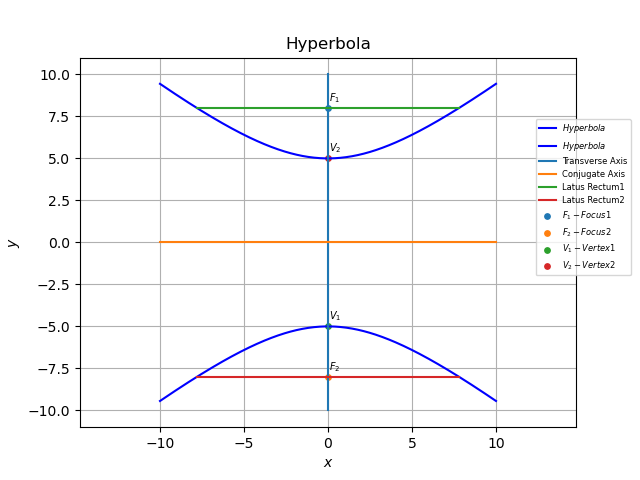
\includegraphics[width=0.75\columnwidth]{chapters/11/11/4/8/figs/hyperbola2}
	\end{center}
\caption{}
\label{fig:chapters/11/11/4/8/Fig1}
\end{figure}

